
\index{Staudinger, M. Ursula}

\paragraph{Research Team}
Team Ursula M. Staudinger (Professor), Eva-Marie Kessler (Doctoral Candidate; graduated 01/2006; postdoctoral fellow), Ines Schindler (Postdoctoral fellow at Utah State University).

This project is interested in processes of developmental regulation during adulthood and old age. Life composition concerns different aspects of self and personality such as emotions, coping, the goal system, and the experience of time. Besides establishing valid measurement for different age groups, we investigate which role these aspects of self and personality play in resilience constellations and the regulation of subjective well-being of old age. 

\null 
\textbf{Research Highlights 2006}

\textit{Personal Life Investment}

 During 2006, work in the area of the goal system (personal life investment, PLI) focused on the distinction between obligatory and optional PLI. PLI is defined as the amount of motivational energy people invest as actions or thoughts in ten central life domains (health, cognitive fitness, hobbies and interests, relationship with friends and acquaintances, sexuality, well-being of relatives, occupation or similar activities, independence, thinking about one's life, death and dying) in order to achieve their personal goals or prevent the loss of prior achievements. Depending on the developmental tasks of a given age period different domains require our obligatory investment and others leave room for optional investments. 

\begin{figure}[htb]
  \begin{center}
    \resizebox{0.4\textwidth}{!}{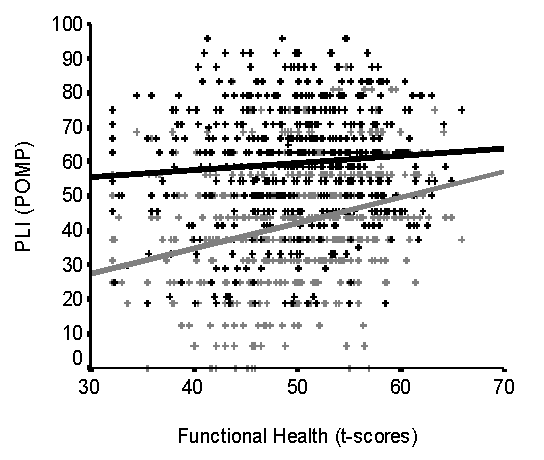
\includegraphics{profUrsulaStaudinger-fig1}}
    \caption{Optional (grey line) and obligatory (black line) as expected differ in their association with levels of objective health. Optional PLI is higher at higher levels of functional health (Schindler \& Staudinger, submitted).}
    \label{fig1:profUrsulaStaudinger}
  \end{center}
\end{figure}


The distinction aims to model the differences between reactive and active types of investments. And indeed, we found that the two types relate differently to indicators of approach and avoidance as well as to indicators of subjective well-being (see Figure \ref{fig1:profUrsulaStaudinger}; Schindler \& Staudinger, submitted). The two types of PLI have demonstrated differential age trajectories in the longitudinal sample of the Berlin Aging Study (Schindler, Staudinger, \& Nesselroade, in press). Across an age range of 30 years and a measurement period of 10 years, optional PLI showed declines and obligatory PLI stayed stable. This finding was replicated when using functional health rather than chronological age as correlate. Obligatory PLI is not related to functional health whereas optional PLI is lower at lower levels of health.

%\begin{figure}[ht]
%  \begin{center}
%    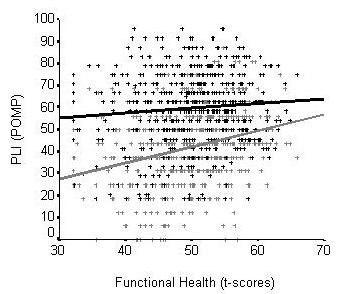
\includegraphics[width=7.5cm]{profUrsulaStaudinger-fig1.png}
%    \caption{Optional (grey line) and obligatory (black line) as expected differ in their association with levels of objective health. Optional PLI is higher at higher levels of functional health (Schindler \& Staudinger, submitted).}\label{fig1:profUrsulaStaudinger}
%   \end{center}
%\end{figure}


Furthermore, in 2006 we conducted a study on the emotional life and its functionality across the lifespan (Kessler \& Staudinger, in preparation). A new emotion questionnaire that assesses the frequency with which certain emotions have been experienced was developed. In contrast to extant questionnaires, the new instrument distinguishes not only between positive and negative emotions but also between emotions that involve high and those that involve low activation. Some of the conflicting patterns of results available in the literature may be related to the lack of this differentiation. And indeed this is what we found: both high and low activated negative emotions decline starting in midlife. Highly activated positive emotions show no age differences, but low activated positive emotions increase starting young adulthood (see Figure \ref{fig2:profUrsulaStaudinger}).

%\begin{figure}[ht]
%  \begin{center}
%    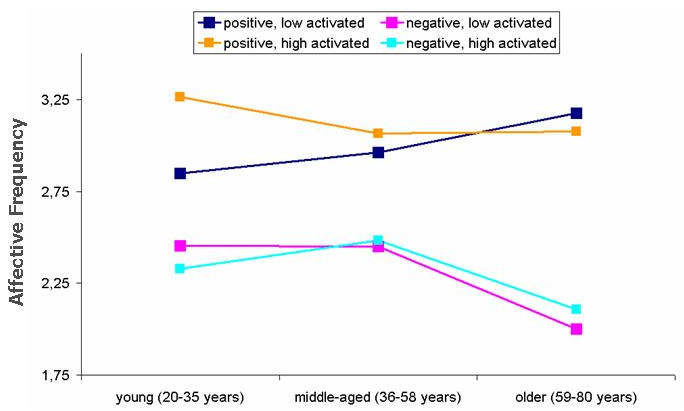
\includegraphics[width=7.5cm]{profUrsulaStaudinger-fig2.png}
%    \caption{Age difference on four facets of emotional life (Kessler \& Staudinger, in preparation).}\label{fig2:profUrsulaStaudinger}
%   \end{center}
%\end{figure}


\begin{figure}[htb]
  \begin{center}
    \resizebox{0.5\textwidth}{!}{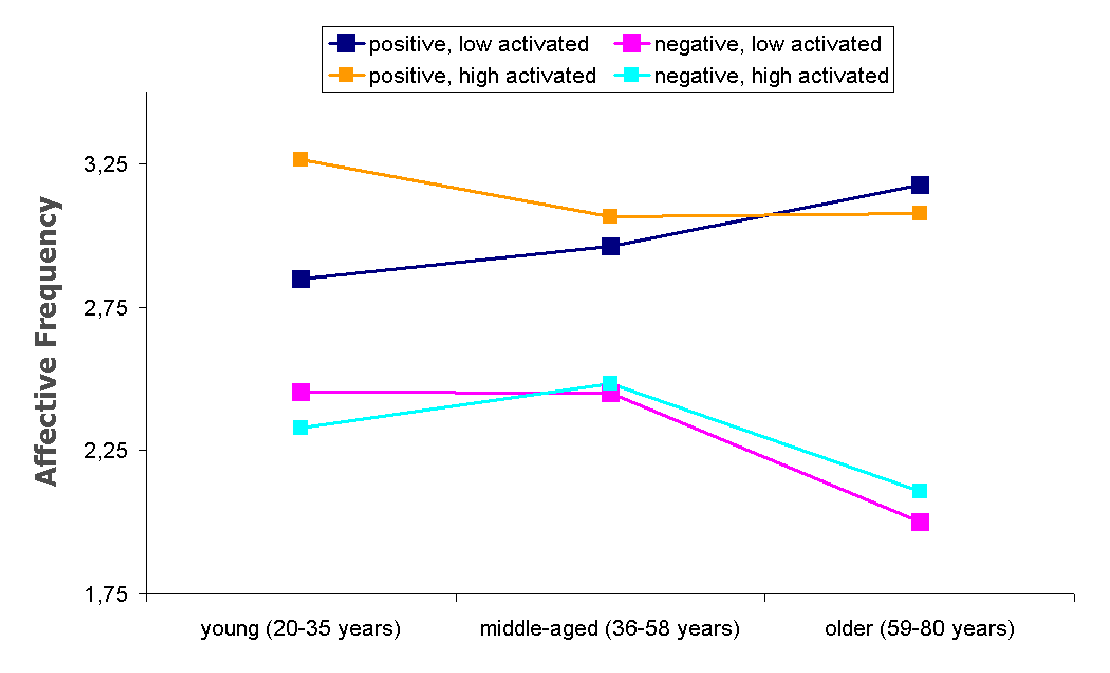
\includegraphics{profUrsulaStaudinger-fig2}}
    \caption{Age difference on four facets of emotional life (Kessler \& Staudinger, in preparation).}
    \label{fig2:profUrsulaStaudinger}
  \end{center}
\end{figure}

\newpage
\paragraph{Collaborations}

\begin{itemize}
\item Brandeis University\\ Prof. Margie Lachman, PhD
\item Stanford University\\ Prof. Laura Carstensen, PhD
\item University Hildesheim\\ Prof. Dr. Werner Greve
\item University of Utah\\ Dr. Ines Schindler
\end{itemize}

\begin{bibunit}[apalike]
\nocite{*}
\putbib[profUrsulaStaudinger2]
\end{bibunit}